\documentclass[1p]{elsarticle_modified}
%\bibliographystyle{elsarticle-num}

%\usepackage[colorlinks]{hyperref}
%\usepackage{abbrmath_seonhwa} %\Abb, \Ascr, \Acal ,\Abf, \Afrak
\usepackage{amsfonts}
\usepackage{amssymb}
\usepackage{amsmath}
\usepackage{amsthm}
\usepackage{scalefnt}
\usepackage{amsbsy}
\usepackage{kotex}
\usepackage{caption}
\usepackage{subfig}
\usepackage{color}
\usepackage{graphicx}
\usepackage{xcolor} %% white, black, red, green, blue, cyan, magenta, yellow
\usepackage{float}
\usepackage{setspace}
\usepackage{hyperref}

\usepackage{tikz}
\usetikzlibrary{arrows}

\usepackage{multirow}
\usepackage{array} % fixed length table
\usepackage{hhline}

%%%%%%%%%%%%%%%%%%%%%
\makeatletter
\renewcommand*\env@matrix[1][\arraystretch]{%
	\edef\arraystretch{#1}%
	\hskip -\arraycolsep
	\let\@ifnextchar\new@ifnextchar
	\array{*\c@MaxMatrixCols c}}
\makeatother %https://tex.stackexchange.com/questions/14071/how-can-i-increase-the-line-spacing-in-a-matrix
%%%%%%%%%%%%%%%

\usepackage[normalem]{ulem}

\newcommand{\msout}[1]{\ifmmode\text{\sout{\ensuremath{#1}}}\else\sout{#1}\fi}
%SOURCE: \msout is \stkout macro in https://tex.stackexchange.com/questions/20609/strikeout-in-math-mode

\newcommand{\cancel}[1]{
	\ifmmode
	{\color{red}\msout{#1}}
	\else
	{\color{red}\sout{#1}}
	\fi
}

\newcommand{\add}[1]{
	{\color{blue}\uwave{#1}}
}

\newcommand{\replace}[2]{
	\ifmmode
	{\color{red}\msout{#1}}{\color{blue}\uwave{#2}}
	\else
	{\color{red}\sout{#1}}{\color{blue}\uwave{#2}}
	\fi
}

\newcommand{\Sol}{\mathcal{S}} %segment
\newcommand{\D}{D} %diagram
\newcommand{\A}{\mathcal{A}} %arc


%%%%%%%%%%%%%%%%%%%%%%%%%%%%%5 test

\def\sl{\operatorname{\textup{SL}}(2,\Cbb)}
\def\psl{\operatorname{\textup{PSL}}(2,\Cbb)}
\def\quan{\mkern 1mu \triangleright \mkern 1mu}

\theoremstyle{definition}
\newtheorem{thm}{Theorem}[section]
\newtheorem{prop}[thm]{Proposition}
\newtheorem{lem}[thm]{Lemma}
\newtheorem{ques}[thm]{Question}
\newtheorem{cor}[thm]{Corollary}
\newtheorem{defn}[thm]{Definition}
\newtheorem{exam}[thm]{Example}
\newtheorem{rmk}[thm]{Remark}
\newtheorem{alg}[thm]{Algorithm}

\newcommand{\I}{\sqrt{-1}}
\begin{document}

%\begin{frontmatter}
%
%\title{Boundary parabolic representations of knots up to 8 crossings}
%
%%% Group authors per affiliation:
%\author{Yunhi Cho} 
%\address{Department of Mathematics, University of Seoul, Seoul, Korea}
%\ead{yhcho@uos.ac.kr}
%
%
%\author{Seonhwa Kim} %\fnref{s_kim}}
%\address{Center for Geometry and Physics, Institute for Basic Science, Pohang, 37673, Korea}
%\ead{ryeona17@ibs.re.kr}
%
%\author{Hyuk Kim}
%\address{Department of Mathematical Sciences, Seoul National University, Seoul 08826, Korea}
%\ead{hyukkim@snu.ac.kr}
%
%\author{Seokbeom Yoon}
%\address{Department of Mathematical Sciences, Seoul National University, Seoul, 08826,  Korea}
%\ead{sbyoon15@snu.ac.kr}
%
%\begin{abstract}
%We find all boundary parabolic representation of knots up to 8 crossings.
%
%\end{abstract}
%\begin{keyword}
%    \MSC[2010] 57M25 
%\end{keyword}
%
%\end{frontmatter}

%\linenumbers
%\tableofcontents
%
\newcommand\colored[1]{\textcolor{white}{\rule[-0.35ex]{0.8em}{1.4ex}}\kern-0.8em\color{red} #1}%
%\newcommand\colored[1]{\textcolor{white}{ #1}\kern-2.17ex	\textcolor{white}{ #1}\kern-1.81ex	\textcolor{white}{ #1}\kern-2.15ex\color{red}#1	}

{\Large $\underline{10_{49}~(K10a_{13})}$}

\setlength{\tabcolsep}{10pt}
\renewcommand{\arraystretch}{1.6}
\vspace{1cm}\begin{tabular}{m{100pt}>{\centering\arraybackslash}m{274pt}}
\multirow{5}{120pt}{
	\centering
	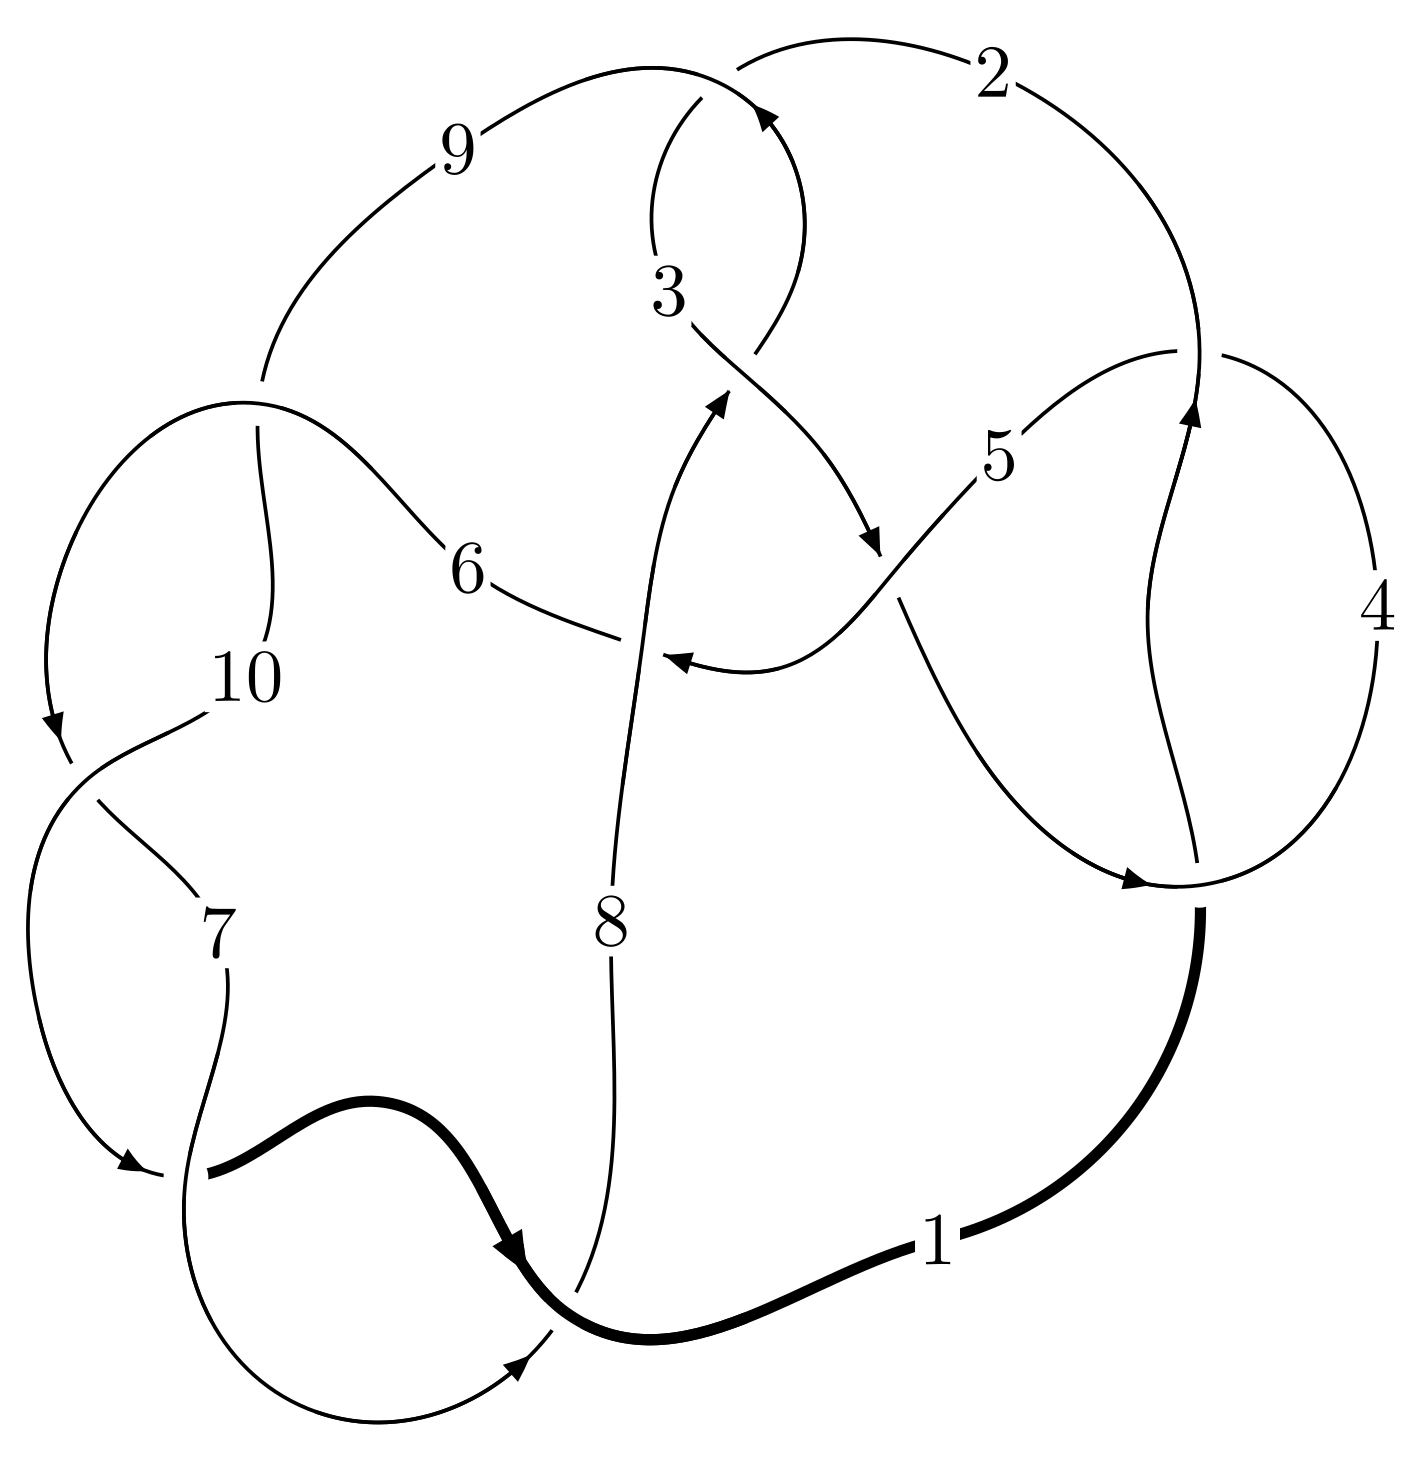
\includegraphics[width=112pt]{../../../GIT/diagram.site/Diagrams/png/133_10_49.png}\\
\ \ \ A knot diagram\footnotemark}&
\allowdisplaybreaks
\textbf{Linearized knot diagam} \\
\cline{2-2}
 &
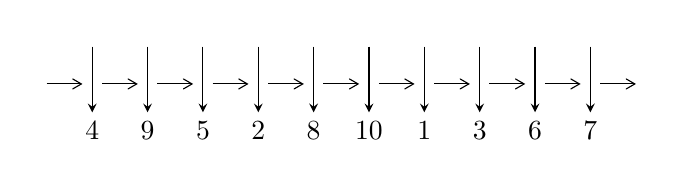
\begin{tikzpicture}[x=20pt, y=17pt]
	% nodes
	\node (C0) at (0, 0) {};
	\node (C1) at (1, 0) {};
	\node (C1U) at (1, +1) {};
	\node (C1D) at (1, -1) {4};

	\node (C2) at (2, 0) {};
	\node (C2U) at (2, +1) {};
	\node (C2D) at (2, -1) {9};

	\node (C3) at (3, 0) {};
	\node (C3U) at (3, +1) {};
	\node (C3D) at (3, -1) {5};

	\node (C4) at (4, 0) {};
	\node (C4U) at (4, +1) {};
	\node (C4D) at (4, -1) {2};

	\node (C5) at (5, 0) {};
	\node (C5U) at (5, +1) {};
	\node (C5D) at (5, -1) {8};

	\node (C6) at (6, 0) {};
	\node (C6U) at (6, +1) {};
	\node (C6D) at (6, -1) {10};

	\node (C7) at (7, 0) {};
	\node (C7U) at (7, +1) {};
	\node (C7D) at (7, -1) {1};

	\node (C8) at (8, 0) {};
	\node (C8U) at (8, +1) {};
	\node (C8D) at (8, -1) {3};

	\node (C9) at (9, 0) {};
	\node (C9U) at (9, +1) {};
	\node (C9D) at (9, -1) {6};

	\node (C10) at (10, 0) {};
	\node (C10U) at (10, +1) {};
	\node (C10D) at (10, -1) {7};
	\node (C11) at (11, 0) {};

	% arrows
	\draw[->,>={angle 60}]
	(C0) edge (C1) (C1) edge (C2) (C2) edge (C3) (C3) edge (C4) (C4) edge (C5) (C5) edge (C6) (C6) edge (C7) (C7) edge (C8) (C8) edge (C9) (C9) edge (C10) (C10) edge (C11) ;	\draw[->,>=stealth]
	(C1U) edge (C1D) (C2U) edge (C2D) (C3U) edge (C3D) (C4U) edge (C4D) (C5U) edge (C5D) (C6U) edge (C6D) (C7U) edge (C7D) (C8U) edge (C8D) (C9U) edge (C9D) (C10U) edge (C10D) ;
	\end{tikzpicture} \\
\hhline{~~} \\& 
\textbf{Solving Sequence} \\ \cline{2-2} 
 &
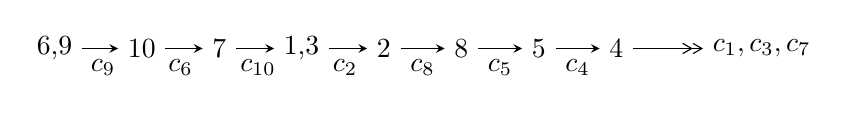
\begin{tikzpicture}[x=28pt, y=7pt]
	% node
	\node (A0) at (-1/8, 0) {6,9};
	\node (A1) at (1, 0) {10};
	\node (A2) at (2, 0) {7};
	\node (A3) at (49/16, 0) {1,3};
	\node (A4) at (33/8, 0) {2};
	\node (A5) at (41/8, 0) {8};
	\node (A6) at (49/8, 0) {5};
	\node (A7) at (57/8, 0) {4};
	\node (C1) at (1/2, -1) {$c_{9}$};
	\node (C2) at (3/2, -1) {$c_{6}$};
	\node (C3) at (5/2, -1) {$c_{10}$};
	\node (C4) at (29/8, -1) {$c_{2}$};
	\node (C5) at (37/8, -1) {$c_{8}$};
	\node (C6) at (45/8, -1) {$c_{5}$};
	\node (C7) at (53/8, -1) {$c_{4}$};
	\node (A8) at (9, 0) {$c_{1},c_{3},c_{7}$};

	% edge
	\draw[->,>=stealth]	
	(A0) edge (A1) (A1) edge (A2) (A2) edge (A3) (A3) edge (A4) (A4) edge (A5) (A5) edge (A6) (A6) edge (A7) ;
	\draw[->>,>={angle 60}]	
	(A7) edge (A8);
\end{tikzpicture} \\ 

\end{tabular} \\

\footnotetext{
The image of knot diagram is generated by the software ``\textbf{Draw programme}" developed by Andrew Bartholomew(\url{http://www.layer8.co.uk/maths/draw/index.htm\#Running-draw}), where we modified some parts for our purpose(\url{https://github.com/CATsTAILs/LinksPainter}).
}\phantom \\ \newline 
\centering \textbf{Ideals for irreducible components\footnotemark of $X_{\text{par}}$} 
 
\begin{align*}
I^u_{1}&=\langle 
- u^{30}+17 u^{28}+\cdots+b-1,\;u^{29}+u^{28}+\cdots+a+1,\;u^{31}+2 u^{30}+\cdots+2 u+1\rangle \\
I^u_{2}&=\langle 
b,\;a- u+1,\;u^2- u-1\rangle \\
\\
\end{align*}
\raggedright * 2 irreducible components of $\dim_{\mathbb{C}}=0$, with total 33 representations.\\
\footnotetext{All coefficients of polynomials are rational numbers. But the coefficients are sometimes approximated in decimal forms when there is not enough margin.}
\newpage
\renewcommand{\arraystretch}{1}
\centering \section*{I. $I^u_{1}= \langle - u^{30}+17 u^{28}+\cdots+b-1,\;u^{29}+u^{28}+\cdots+a+1,\;u^{31}+2 u^{30}+\cdots+2 u+1 \rangle$}
\flushleft \textbf{(i) Arc colorings}\\
\begin{tabular}{m{7pt} m{180pt} m{7pt} m{180pt} }
\flushright $a_{6}=$&$\begin{pmatrix}0\\u\end{pmatrix}$ \\
\flushright $a_{9}=$&$\begin{pmatrix}1\\0\end{pmatrix}$ \\
\flushright $a_{10}=$&$\begin{pmatrix}1\\u^2\end{pmatrix}$ \\
\flushright $a_{7}=$&$\begin{pmatrix}- u\\- u^3+u\end{pmatrix}$ \\
\flushright $a_{1}=$&$\begin{pmatrix}- u^2+1\\- u^4+2 u^2\end{pmatrix}$ \\
\flushright $a_{3}=$&$\begin{pmatrix}- u^{29}- u^{28}+\cdots- u-1\\u^{30}-17 u^{28}+\cdots+3 u+1\end{pmatrix}$ \\
\flushright $a_{2}=$&$\begin{pmatrix}u^{30}- u^{29}+\cdots-3 u^2+2 u\\u^{30}-17 u^{28}+\cdots+3 u+1\end{pmatrix}$ \\
\flushright $a_{8}=$&$\begin{pmatrix}u^3-2 u\\u^5-3 u^3+u\end{pmatrix}$ \\
\flushright $a_{5}=$&$\begin{pmatrix}u^7-4 u^5+4 u^3\\u^9-5 u^7+7 u^5-2 u^3+u\end{pmatrix}$ \\
\flushright $a_{4}=$&$\begin{pmatrix}- u^{29}- u^{28}+\cdots- u^2+u\\- u^{14}+8 u^{12}+\cdots+u^2+2 u\end{pmatrix}$\\&\end{tabular}
\flushleft \textbf{(ii) Obstruction class $= -1$}\\~\\
\flushleft \textbf{(iii) Cusp Shapes $= 4 u^{30}+3 u^{29}-63 u^{28}-42 u^{27}+425 u^{26}+231 u^{25}-1601 u^{24}-582 u^{23}+3678 u^{22}+378 u^{21}-5240 u^{20}+1434 u^{19}+4267 u^{18}-3741 u^{17}-861 u^{16}+3662 u^{15}-2258 u^{14}-1402 u^{13}+2636 u^{12}-406 u^{11}-1210 u^{10}+852 u^9+292 u^8-384 u^7+86 u^6+142 u^5-32 u^4-6 u^3+13 u^2+9 u-11$}\\~\\
\newpage\renewcommand{\arraystretch}{1}
\flushleft \textbf{(iv) u-Polynomials at the component}\newline \\
\begin{tabular}{m{50pt}|m{274pt}}
Crossings & \hspace{64pt}u-Polynomials at each crossing \\
\hline $$\begin{aligned}c_{1},c_{4}\end{aligned}$$&$\begin{aligned}
&u^{31}-3 u^{30}+\cdots+3 u+1
\end{aligned}$\\
\hline $$\begin{aligned}c_{2},c_{8}\end{aligned}$$&$\begin{aligned}
&u^{31}+u^{30}+\cdots+12 u+4
\end{aligned}$\\
\hline $$\begin{aligned}c_{3}\end{aligned}$$&$\begin{aligned}
&u^{31}+15 u^{30}+\cdots+29 u+1
\end{aligned}$\\
\hline $$\begin{aligned}c_{5}\end{aligned}$$&$\begin{aligned}
&u^{31}-8 u^{30}+\cdots+14 u+7
\end{aligned}$\\
\hline $$\begin{aligned}c_{6},c_{7},c_{9}\\c_{10}\end{aligned}$$&$\begin{aligned}
&u^{31}+2 u^{30}+\cdots+2 u+1
\end{aligned}$\\
\hline
\end{tabular}\\~\\
\newpage\renewcommand{\arraystretch}{1}
\flushleft \textbf{(v) Riley Polynomials at the component}\newline \\
\begin{tabular}{m{50pt}|m{274pt}}
Crossings & \hspace{64pt}Riley Polynomials at each crossing \\
\hline $$\begin{aligned}c_{1},c_{4}\end{aligned}$$&$\begin{aligned}
&y^{31}-15 y^{30}+\cdots+29 y-1
\end{aligned}$\\
\hline $$\begin{aligned}c_{2},c_{8}\end{aligned}$$&$\begin{aligned}
&y^{31}+15 y^{30}+\cdots-8 y-16
\end{aligned}$\\
\hline $$\begin{aligned}c_{3}\end{aligned}$$&$\begin{aligned}
&y^{31}+5 y^{30}+\cdots+505 y-1
\end{aligned}$\\
\hline $$\begin{aligned}c_{5}\end{aligned}$$&$\begin{aligned}
&y^{31}+20 y^{29}+\cdots-602 y-49
\end{aligned}$\\
\hline $$\begin{aligned}c_{6},c_{7},c_{9}\\c_{10}\end{aligned}$$&$\begin{aligned}
&y^{31}-36 y^{30}+\cdots+10 y-1
\end{aligned}$\\
\hline
\end{tabular}\\~\\
\newpage\flushleft \textbf{(vi) Complex Volumes and Cusp Shapes}
$$\begin{array}{c|c|c}  
\text{Solutions to }I^u_{1}& \I (\text{vol} + \sqrt{-1}CS) & \text{Cusp shape}\\
 \hline 
\begin{aligned}
u &= -0.942627 + 0.191065 I \\
a &= -0.160124 + 0.103064 I \\
b &= \phantom{-}0.324783 + 0.959750 I\end{aligned}
 & -1.73768 - 1.98261 I & -12.51789 + 2.95931 I \\ \hline\begin{aligned}
u &= -0.942627 - 0.191065 I \\
a &= -0.160124 - 0.103064 I \\
b &= \phantom{-}0.324783 - 0.959750 I\end{aligned}
 & -1.73768 + 1.98261 I & -12.51789 - 2.95931 I \\ \hline\begin{aligned}
u &= \phantom{-}0.696545 + 0.545292 I \\
a &= \phantom{-}1.23592 - 1.62736 I \\
b &= \phantom{-}0.613275 + 1.178920 I\end{aligned}
 & \phantom{-}0.71112 - 8.80296 I & -11.07196 + 8.43090 I \\ \hline\begin{aligned}
u &= \phantom{-}0.696545 - 0.545292 I \\
a &= \phantom{-}1.23592 + 1.62736 I \\
b &= \phantom{-}0.613275 - 1.178920 I\end{aligned}
 & \phantom{-}0.71112 + 8.80296 I & -11.07196 - 8.43090 I \\ \hline\begin{aligned}
u &= \phantom{-}0.605327 + 0.533968 I \\
a &= -1.15171 + 1.76364 I \\
b &= -0.398966 - 1.160740 I\end{aligned}
 & \phantom{-}2.77360 - 3.43811 I & -7.57029 + 4.39561 I \\ \hline\begin{aligned}
u &= \phantom{-}0.605327 - 0.533968 I \\
a &= -1.15171 - 1.76364 I \\
b &= -0.398966 + 1.160740 I\end{aligned}
 & \phantom{-}2.77360 + 3.43811 I & -7.57029 - 4.39561 I \\ \hline\begin{aligned}
u &= -0.605796 + 0.419305 I \\
a &= -0.106041 + 0.538372 I \\
b &= \phantom{-}0.914628 + 0.393426 I\end{aligned}
 & -1.75392 + 3.16934 I & -13.1405 - 6.2492 I \\ \hline\begin{aligned}
u &= -0.605796 - 0.419305 I \\
a &= -0.106041 - 0.538372 I \\
b &= \phantom{-}0.914628 - 0.393426 I\end{aligned}
 & -1.75392 - 3.16934 I & -13.1405 + 6.2492 I \\ \hline\begin{aligned}
u &= \phantom{-}0.216063 + 0.636597 I \\
a &= \phantom{-}0.53700 - 1.67610 I \\
b &= -0.488198 + 1.161550 I\end{aligned}
 & \phantom{-}2.12474 + 4.80226 I & -7.72031 - 3.44347 I \\ \hline\begin{aligned}
u &= \phantom{-}0.216063 - 0.636597 I \\
a &= \phantom{-}0.53700 + 1.67610 I \\
b &= -0.488198 - 1.161550 I\end{aligned}
 & \phantom{-}2.12474 - 4.80226 I & -7.72031 + 3.44347 I\\
 \hline 
 \end{array}$$\newpage$$\begin{array}{c|c|c}  
\text{Solutions to }I^u_{1}& \I (\text{vol} + \sqrt{-1}CS) & \text{Cusp shape}\\
 \hline 
\begin{aligned}
u &= \phantom{-}0.331449 + 0.582530 I \\
a &= -0.68223 + 1.81325 I \\
b &= \phantom{-}0.208622 - 1.161580 I\end{aligned}
 & \phantom{-}3.57659 - 0.38668 I & -5.31318 + 2.65084 I \\ \hline\begin{aligned}
u &= \phantom{-}0.331449 - 0.582530 I \\
a &= -0.68223 - 1.81325 I \\
b &= \phantom{-}0.208622 + 1.161580 I\end{aligned}
 & \phantom{-}3.57659 + 0.38668 I & -5.31318 - 2.65084 I \\ \hline\begin{aligned}
u &= \phantom{-}0.574643 + 0.305412 I \\
a &= \phantom{-}1.51598 - 2.33460 I \\
b &= \phantom{-}0.313373 + 0.704732 I\end{aligned}
 & -2.56499 - 0.98527 I & -12.14842 + 6.83319 I \\ \hline\begin{aligned}
u &= \phantom{-}0.574643 - 0.305412 I \\
a &= \phantom{-}1.51598 + 2.33460 I \\
b &= \phantom{-}0.313373 - 0.704732 I\end{aligned}
 & -2.56499 + 0.98527 I & -12.14842 - 6.83319 I \\ \hline\begin{aligned}
u &= -1.400590 + 0.076803 I \\
a &= \phantom{-}0.284363 + 0.723650 I \\
b &= \phantom{-}0.076838 - 1.243230 I\end{aligned}
 & -1.80597 + 2.68803 I & -9.99041 - 3.16248 I \\ \hline\begin{aligned}
u &= -1.400590 - 0.076803 I \\
a &= \phantom{-}0.284363 - 0.723650 I \\
b &= \phantom{-}0.076838 + 1.243230 I\end{aligned}
 & -1.80597 - 2.68803 I & -9.99041 + 3.16248 I \\ \hline\begin{aligned}
u &= \phantom{-}1.54559 + 0.05817 I \\
a &= \phantom{-}0.500839 - 0.189268 I \\
b &= \phantom{-}0.922872 - 0.250964 I\end{aligned}
 & -7.37189 - 0.63906 I & -13.31985 + 0. I\phantom{ +0.000000I} \\ \hline\begin{aligned}
u &= \phantom{-}1.54559 - 0.05817 I \\
a &= \phantom{-}0.500839 + 0.189268 I \\
b &= \phantom{-}0.922872 + 0.250964 I\end{aligned}
 & -7.37189 + 0.63906 I & -13.31985 + 0. I\phantom{ +0.000000I} \\ \hline\begin{aligned}
u &= -0.283148 + 0.347355 I \\
a &= -0.301800 - 0.948705 I \\
b &= -0.732891 + 0.139904 I\end{aligned}
 & -0.846644 - 0.285966 I & -10.27924 - 1.27611 I \\ \hline\begin{aligned}
u &= -0.283148 - 0.347355 I \\
a &= -0.301800 + 0.948705 I \\
b &= -0.732891 - 0.139904 I\end{aligned}
 & -0.846644 + 0.285966 I & -10.27924 + 1.27611 I\\
 \hline 
 \end{array}$$\newpage$$\begin{array}{c|c|c}  
\text{Solutions to }I^u_{1}& \I (\text{vol} + \sqrt{-1}CS) & \text{Cusp shape}\\
 \hline 
\begin{aligned}
u &= -0.440544\phantom{ +0.000000I} \\
a &= -0.456355\phantom{ +0.000000I} \\
b &= -0.447925\phantom{ +0.000000I}\end{aligned}
 & -0.703249\phantom{ +0.000000I} & -13.8910\phantom{ +0.000000I} \\ \hline\begin{aligned}
u &= -1.56849 + 0.15264 I \\
a &= \phantom{-}1.094690 + 0.849273 I \\
b &= \phantom{-}0.557583 - 1.179560 I\end{aligned}
 & -4.51872 + 5.93011 I & -10.96804 - 3.41229 I \\ \hline\begin{aligned}
u &= -1.56849 - 0.15264 I \\
a &= \phantom{-}1.094690 - 0.849273 I \\
b &= \phantom{-}0.557583 + 1.179560 I\end{aligned}
 & -4.51872 - 5.93011 I & -10.96804 + 3.41229 I \\ \hline\begin{aligned}
u &= -1.57353 + 0.09063 I \\
a &= -1.14209 - 1.28668 I \\
b &= -0.446370 + 0.932965 I\end{aligned}
 & -9.92171 + 2.45212 I & -15.0553 - 2.8825 I \\ \hline\begin{aligned}
u &= -1.57353 - 0.09063 I \\
a &= -1.14209 + 1.28668 I \\
b &= -0.446370 - 0.932965 I\end{aligned}
 & -9.92171 - 2.45212 I & -15.0553 + 2.8825 I \\ \hline\begin{aligned}
u &= \phantom{-}1.57590 + 0.11764 I \\
a &= -0.484278 + 0.374146 I \\
b &= -1.031430 + 0.523808 I\end{aligned}
 & -9.15652 - 5.11817 I & -15.5151 + 3.8713 I \\ \hline\begin{aligned}
u &= \phantom{-}1.57590 - 0.11764 I \\
a &= -0.484278 - 0.374146 I \\
b &= -1.031430 - 0.523808 I\end{aligned}
 & -9.15652 + 5.11817 I & -15.5151 - 3.8713 I \\ \hline\begin{aligned}
u &= -1.60251 + 0.16367 I \\
a &= -1.24549 - 0.75908 I \\
b &= -0.711416 + 1.179640 I\end{aligned}
 & -7.05058 + 11.45320 I & -13.9714 - 7.0213 I \\ \hline\begin{aligned}
u &= -1.60251 - 0.16367 I \\
a &= -1.24549 + 0.75908 I \\
b &= -0.711416 - 1.179640 I\end{aligned}
 & -7.05058 - 11.45320 I & -13.9714 + 7.0213 I \\ \hline\begin{aligned}
u &= \phantom{-}1.65145 + 0.04258 I \\
a &= -0.166851 + 0.356098 I \\
b &= -0.398737 + 0.726247 I\end{aligned}
 & -10.63140 + 1.14909 I & -14.4727 - 5.7136 I\\
 \hline 
 \end{array}$$\newpage$$\begin{array}{c|c|c}  
\text{Solutions to }I^u_{1}& \I (\text{vol} + \sqrt{-1}CS) & \text{Cusp shape}\\
 \hline 
\begin{aligned}
u &= \phantom{-}1.65145 - 0.04258 I \\
a &= -0.166851 - 0.356098 I \\
b &= -0.398737 - 0.726247 I\end{aligned}
 & -10.63140 - 1.14909 I & -14.4727 + 5.7136 I\\
 \hline 
 \end{array}$$\newpage\newpage\renewcommand{\arraystretch}{1}
\centering \section*{II. $I^u_{2}= \langle b,\;a- u+1,\;u^2- u-1 \rangle$}
\flushleft \textbf{(i) Arc colorings}\\
\begin{tabular}{m{7pt} m{180pt} m{7pt} m{180pt} }
\flushright $a_{6}=$&$\begin{pmatrix}0\\u\end{pmatrix}$ \\
\flushright $a_{9}=$&$\begin{pmatrix}1\\0\end{pmatrix}$ \\
\flushright $a_{10}=$&$\begin{pmatrix}1\\u+1\end{pmatrix}$ \\
\flushright $a_{7}=$&$\begin{pmatrix}- u\\- u-1\end{pmatrix}$ \\
\flushright $a_{1}=$&$\begin{pmatrix}- u\\- u\end{pmatrix}$ \\
\flushright $a_{3}=$&$\begin{pmatrix}u-1\\0\end{pmatrix}$ \\
\flushright $a_{2}=$&$\begin{pmatrix}u-1\\0\end{pmatrix}$ \\
\flushright $a_{8}=$&$\begin{pmatrix}1\\0\end{pmatrix}$ \\
\flushright $a_{5}=$&$\begin{pmatrix}u\\u\end{pmatrix}$ \\
\flushright $a_{4}=$&$\begin{pmatrix}2 u-1\\u\end{pmatrix}$\\&\end{tabular}
\flushleft \textbf{(ii) Obstruction class $= 1$}\\~\\
\flushleft \textbf{(iii) Cusp Shapes $= -15$}\\~\\
\newpage\renewcommand{\arraystretch}{1}
\flushleft \textbf{(iv) u-Polynomials at the component}\newline \\
\begin{tabular}{m{50pt}|m{274pt}}
Crossings & \hspace{64pt}u-Polynomials at each crossing \\
\hline $$\begin{aligned}c_{1},c_{3}\end{aligned}$$&$\begin{aligned}
&(u-1)^2
\end{aligned}$\\
\hline $$\begin{aligned}c_{2},c_{8}\end{aligned}$$&$\begin{aligned}
&u^2
\end{aligned}$\\
\hline $$\begin{aligned}c_{4}\end{aligned}$$&$\begin{aligned}
&(u+1)^2
\end{aligned}$\\
\hline $$\begin{aligned}c_{5},c_{6},c_{7}\end{aligned}$$&$\begin{aligned}
&u^2+u-1
\end{aligned}$\\
\hline $$\begin{aligned}c_{9},c_{10}\end{aligned}$$&$\begin{aligned}
&u^2- u-1
\end{aligned}$\\
\hline
\end{tabular}\\~\\
\newpage\renewcommand{\arraystretch}{1}
\flushleft \textbf{(v) Riley Polynomials at the component}\newline \\
\begin{tabular}{m{50pt}|m{274pt}}
Crossings & \hspace{64pt}Riley Polynomials at each crossing \\
\hline $$\begin{aligned}c_{1},c_{3},c_{4}\end{aligned}$$&$\begin{aligned}
&(y-1)^2
\end{aligned}$\\
\hline $$\begin{aligned}c_{2},c_{8}\end{aligned}$$&$\begin{aligned}
&y^2
\end{aligned}$\\
\hline $$\begin{aligned}c_{5},c_{6},c_{7}\\c_{9},c_{10}\end{aligned}$$&$\begin{aligned}
&y^2-3 y+1
\end{aligned}$\\
\hline
\end{tabular}\\~\\
\newpage\flushleft \textbf{(vi) Complex Volumes and Cusp Shapes}
$$\begin{array}{c|c|c}  
\text{Solutions to }I^u_{2}& \I (\text{vol} + \sqrt{-1}CS) & \text{Cusp shape}\\
 \hline 
\begin{aligned}
u &= -0.618034\phantom{ +0.000000I} \\
a &= -1.61803\phantom{ +0.000000I} \\
b &= \phantom{-0.000000 } 0\end{aligned}
 & -2.63189\phantom{ +0.000000I} & -15.0000\phantom{ +0.000000I} \\ \hline\begin{aligned}
u &= \phantom{-}1.61803\phantom{ +0.000000I} \\
a &= \phantom{-}0.618034\phantom{ +0.000000I} \\
b &= \phantom{-0.000000 } 0\end{aligned}
 & -10.5276\phantom{ +0.000000I} & -15.0000\phantom{ +0.000000I}\\
 \hline 
 \end{array}$$\newpage
\newpage\renewcommand{\arraystretch}{1}
\centering \section*{ III. u-Polynomials}
\begin{tabular}{m{50pt}|m{274pt}}
Crossings & \hspace{64pt}u-Polynomials at each crossing \\
\hline $$\begin{aligned}c_{1}\end{aligned}$$&$\begin{aligned}
&((u-1)^2)(u^{31}-3 u^{30}+\cdots+3 u+1)
\end{aligned}$\\
\hline $$\begin{aligned}c_{2},c_{8}\end{aligned}$$&$\begin{aligned}
&u^2(u^{31}+u^{30}+\cdots+12 u+4)
\end{aligned}$\\
\hline $$\begin{aligned}c_{3}\end{aligned}$$&$\begin{aligned}
&((u-1)^2)(u^{31}+15 u^{30}+\cdots+29 u+1)
\end{aligned}$\\
\hline $$\begin{aligned}c_{4}\end{aligned}$$&$\begin{aligned}
&((u+1)^2)(u^{31}-3 u^{30}+\cdots+3 u+1)
\end{aligned}$\\
\hline $$\begin{aligned}c_{5}\end{aligned}$$&$\begin{aligned}
&(u^2+u-1)(u^{31}-8 u^{30}+\cdots+14 u+7)
\end{aligned}$\\
\hline $$\begin{aligned}c_{6},c_{7}\end{aligned}$$&$\begin{aligned}
&(u^2+u-1)(u^{31}+2 u^{30}+\cdots+2 u+1)
\end{aligned}$\\
\hline $$\begin{aligned}c_{9},c_{10}\end{aligned}$$&$\begin{aligned}
&(u^2- u-1)(u^{31}+2 u^{30}+\cdots+2 u+1)
\end{aligned}$\\
\hline
\end{tabular}\newpage\renewcommand{\arraystretch}{1}
\centering \section*{ IV. Riley Polynomials}
\begin{tabular}{m{50pt}|m{274pt}}
Crossings & \hspace{64pt}Riley Polynomials at each crossing \\
\hline $$\begin{aligned}c_{1},c_{4}\end{aligned}$$&$\begin{aligned}
&((y-1)^2)(y^{31}-15 y^{30}+\cdots+29 y-1)
\end{aligned}$\\
\hline $$\begin{aligned}c_{2},c_{8}\end{aligned}$$&$\begin{aligned}
&y^2(y^{31}+15 y^{30}+\cdots-8 y-16)
\end{aligned}$\\
\hline $$\begin{aligned}c_{3}\end{aligned}$$&$\begin{aligned}
&((y-1)^2)(y^{31}+5 y^{30}+\cdots+505 y-1)
\end{aligned}$\\
\hline $$\begin{aligned}c_{5}\end{aligned}$$&$\begin{aligned}
&(y^2-3 y+1)(y^{31}+20 y^{29}+\cdots-602 y-49)
\end{aligned}$\\
\hline $$\begin{aligned}c_{6},c_{7},c_{9}\\c_{10}\end{aligned}$$&$\begin{aligned}
&(y^2-3 y+1)(y^{31}-36 y^{30}+\cdots+10 y-1)
\end{aligned}$\\
\hline
\end{tabular}
\vskip 2pc
\end{document}